
% Take extra care in avoiding ``expansion'' -- stick to ``evaluation''

\begin{abstract}
Despite the recent improvements in admissible heuristic search techniques
in classical planning, it is known that the the exponential growth of
search plateau in A* is unavoidable even under the optimistic assumption.
 % 
We investigate various existing myth on tiebreaking
strategies and propose simple yet effective methods for improving the
search performance within plateau.
 % 
 % 
 They do not depend on any particular heuristic, nor
 on multi-heuristic portfolio.
 They work even if the heuristic
 function no longer provides useful information.
 % Moreover, they do not even try to obtain any further information from
 % the domain.
 We empirically evaluate our strategies against state-of-the-art admissible planner.
\end{abstract}

\section{Introduction}
%Motivation: The Importance of the Last Frontier in A* and Domains with Large Plateaus
\label{sec-1}



%\subsubparagraph{\astar and perfect heuristics}

This paper investigates tie-breaking strategies for \astar.
\astar is a standard search algorithm for finding an optimal-cost path 
from an initial state $s$ to some goal state $g \in G$ in a search space represented as a graph \cite{hart1968formal}.
In each iteration, \astar selects and \emph{expands} a node $n$ from the OPEN priority queue.
\astar selects and expands the node which has the lowest $f$-cost, where for node $n$, $f(n)$ is the sum of  $g(n)$, the cost of the current path from the start state to $n$, and $h(n)$, a heuristic estimate of the cost from $n$ to a goal state.
\astar returns an optimal solution when $h$ is admissible, i.e., when it
never overestimates the true distance to the goal $h^*$.

In order to guarantee solution optimality, \astar expands all
nodes with $f(n) < f^*$, where $f^*$ is the cost of the optimal solution.
%All nodes with $f(n) = k$ are expanded before any node with $f(n) > k$ are expanded.
%Thus, after all nodes with $f(n) < f^*$ have been expanded, 
\astar expands \emph{some} of the nodes with $f(n) = f^*$, and never expands a node with $f(n) > f^*$.
Thus, the \emph{effective search space of \astar}, $N$, is the set of nodes with 
$f(n) \leq f^*$, and
much of the work in the AI search and planning literature  has focused on reducing the size of $N$ by
developing more accurate, admissible heuristic functions.

In many problems, the size of the \emph{last frontier}, the set of nodes with $f(n)=f^*$, accounts for a significant portion of $A$.
\refig{fig:plateau-noh} plots the number of states with $f(n) = f^*$ (y-axis)
versus the number of states with $f(n) \leq f^*$
for a set of 1104 benchmark problem instances from the ICAPS International Planning Competition (IPC1998-2011).
For many instances in \refig{fig:plateau-noh},  a large fraction of the nodes with $f(n) \leq f^*$ have $f(n)=f^*$.
For example, in the Openstacks domain, almost all states with $f(n) \leq f^*$ have cost $f^*$.
In such domains, the behavior of \astar on the last frontier is critical -- the policy for deciding which nodes to expand in the last frontier can have a significant impact on the performance of \astar.

\begin{figure}[htb]
 \centering \relsize{-3} 
 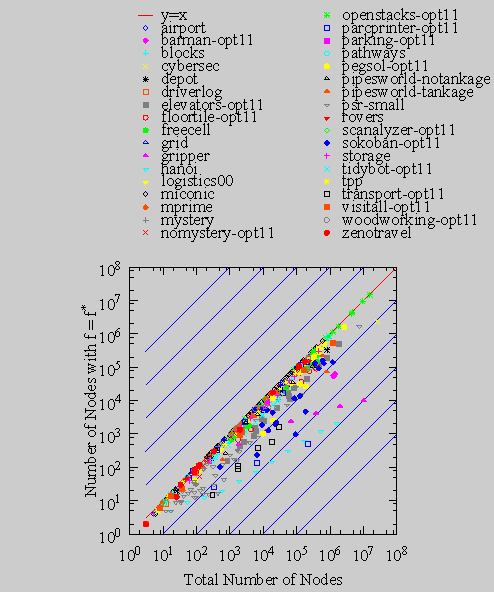
\includegraphics{tables/aaai16-frontier/aaai16prelim3/lmcut_frontier_noh-front.pdf}
 \caption{
 The number of the nodes with cost $f=f^*$ (y-axis) compared to the
 total number of nodes in the search space with cost $f\leq f^*$ on 1104 IPC benchmark problems
(search space analyzed using Fast Downward with \lmcut heuristic, slightly modified to generate all nodes with cost $f^*$).}
\label{fig:plateau-noh}
\end{figure}

In this paper, we focus on the \emph{tie-breaking} policy used by \astar, which selects a node to expand among nodes with the same $f$-cost.
Since \astar expandes all nodes with $f$-cost less than $f^*$ before expanding any nodes with with cost $f^*$, 
the tie-breaking poicy only affects performance when considering the last frontier (nodes with cost $f^*$).
Although there has not been much previous \emph{in-depth} work on tie-breaking policies,
it is widely believed that among nodes with cost $f(n) = f^*$, ties should be broken according to $h(n)$, i.e., nodes with smaller $h$ values should be expanded first.
While this is a useful rule of thumb in many domains,
it turns out that tie-breaking requires more careful consideration, particularly for problems with large \emph{plateaus} -- regions of the search space with the same cost.
\emph{Note that all tiebreaking strategies investigated in this paper maintain the admissibility of the search
because only the node expansion order among nodes that share the same $f$-cost are affected.}

We first show several important findings regarding the
existing tiebreaking strategy for \astar as follows.
% 
First, in implementing the open list of \astar, priority queue which holds
LIFO-buckets for each $f$ is more efficient than that holds FIFO-buckets.
% 
Second, with LIFO-based implementation, $h$-based tiebreaking which
frequently appears in the heuristic search literatures have little
impact on the performance.
% 
\todo[
Third, the LIFO-based bucket implementation and $h$-based tiebreaking
both share the greedy search pattern within the plateau of the
search space.]{this is not shown yet}

Next, based on these observations, we propose three tiebreaking methods
based on the \emph{depth} within the plateau.  From this result, we show
that the performance of above LIFO tiebreaking can be explained by its
depth-first strategy and not by the machine-level efficiency of LIFO
implementation itself.  Also, the performance comparison of different
depth-based strategies showed that they are not dominating each other.

Finally, based on the absence of dominance relationship, we propose a
new class of portfolio strategy which alternates between several
tiebreaking methods.
% 
With this portfolio strategy,
the number of evaluations of nodes with $f<f*$ is exactly the same as
in any single tiebreaking strategies.
Also, it has a theoretical guarantee that
the number of evaluations of nodes with $f=f*$ is at most $N$ times the \emph{minimum} 
of the evaluations required by $N$ strategies in the portfolio.
To put it simply, this portfolio does not need additional computation
and we get a speedup for free (aside from the negligeble differences).
% Also, it is characteristic in that it works with a single heuristic function.




\section{Tie-breaking Strategies in \astar}

%Aside from the heuristic function, most best-first family of search
%algorithms, including \astar, IDA* and so on, have a tiebreaking criteria which is used
%when two nodes have the same $f$ value.

If multiple nodes with the same $f$-cost are possible, \astar
must implement some tie-breaking policy (either
explicitly or implicitly) in order to select from among these nodes.
In practice, tie-breaking based on the $h$-value (breaking ties in favor of nodes with higher $h$) is almost universally used.
As far as we are aware, $h$-based tie-breaking is ``folklore'' in the heuristic search literature.
The original paper proposing \astar paper, as well as Nilsson's subsequent textbook states: ``Select the open node $n$ whose value $f$ is smallest. Resolve ties arbitrarily, but always in favor of any [goal node]'' (\cite{hart1968formal},p.102 Step 2, \cite{Nilsson71}, p.69). % [goal node] : actual text is $n \in T$.
Although it is possible to interpret this to imply $h$-based tie-breaking, since goal nodes are a special case where $h=0$, 
they make no further metion of tie-breaking.
Pearl's seminal textbook on search specifies that best-first search should ``break ties arbitrarily'' (\citeyear{pearl1984heuristics}, p.48, Step 3), but does not specifically mention tie-breaking for \astar.
Thus, the early literature on heuristic search seems to have been mostly agnostic on the issue of tie-breaking.
Interestingly, in his analysis of IDA*, Korf mentions that ``If \astar employs the tie-breaking rule of 'most-recently generated', it must also expand the same nodes [as IDA*]'' (\citeyear{korf1985depth}) -- this Last-In-First-Out ordering is the first explicit mention we found of a tie-breaking policy not based on $h$.

In recent years, tie-breaking accoording to $h$-values has become ``folklore'' in the search community.
\citeauthor{hansen2007anytime} state that ``It is well-known 
that \astar achieves best performance when it breaks ties
in favor of nodes with least h-cost'' \cite{hansen2007anytime}.
\citeauthor{holte2010common} writes ``\astar breaks ties in favour
of larger g values, as is most often done'' (note that since $f=g+h$, preferring large $g$ is equivalent to preferring large $h$).
% \citeauthor{felner2011inconsistent} also assume ``ties are broken in
% favor of low h-values'' in describing Bidirectional Pathmax for \astar.
In their detailed survey/tutorial of efficient \astar implementations, \citeauthor{burns2012implementing} also break ties ``preferring high
$g$.'' They further write: ``The reasoning is that the goal can be found more quickly in the final $f$ layer of search''. 
Thus, tie-breaking according to $h$-values appears to be ubiquitous in practice.


Although the standard practice of tie-breaking according to $h$ might be sufficient in some domains, further levels of tie-breaking (explicit or implicit) are required if multiple nodes can have the same $f$ and $h$ values.
We are not aware of any work that explicitly mentions 2nd-level tie-breaking.
While the survey of efficient \astar implementatins in \citeauthor{burns2012implementing} did not explicitly mention 2nd-level tie-breaking, their code first breaks ties according to $h$, and then breaks remaining ties according to a Last-In-First-Out (LIFO) policy (most recently generated nodes first).\footnote{https://github.com/eaburns/search}
Their choice of a LIFO 2nd-level tie-breaking policy appears to be a natural consequence of the fact that the LIFO policy can be trivially, efficiently implemented in their two-level bucket (vector) implementation of their OPEN list.
In contrast, the current implementation of \sota \astar based planner Fast
Downward \cite{Helmert2006}\footnote{http://www.fast-downward.org} uses a First-In-First-Out (FIFO) second-level tie-breaking policy. We could not find any documentation for this choice. 

%\citeauthor{Korf1985depth} uses $h$-based tiebreaking in the context of WA*
%\cite{korf1993linear}.  
% ** not sure how/where to put this..

\subsection{Evaluation of Two-Level Tie-Breaking Strategies}


We tested various tiebreaking strategies. In the following sections, we
use a convenient array-based notation of a combination of tiebreaking
strategy.  For example, $[f,h,\fd,\fifo]$ denotes standard \astar with
$h$-based first-level tiebreaking, FirstDepth second-level tiebreaking and FIFO
third-level tiebreaking.

All planners are based on the latest Fast Downward code base, and all
experiments are run using 30 minutes runtime cutoff with 2GB memory
limit. Experiments were conducted on Xeon E5410@2.33GHz CPUs.
Our experimental results include 28 standard benchmark domains with 1104
problems

We first compared three strategies 
$[f,h,\fifo]$, $[f,h,\lifo]$ and $[f,h,\ro]$, 
which first breaks ties according to $h$, and then applies \fifo, \lifo, or \ro second-level tie-breaking, respectively.
The results (for \astar using the LM-cut heuristic \cite{Helmert2009}) are shown 
 in \reftbl{single-coverage} (Left).  Differences in coverage can be overved in several domains.
Due to the space limitation, we show only the domains
where the difference was observed. Full data is available in the
supplemental material. \todo{probably better to show full results for this particular experiment}.

Although the search behavior of $[f,h,\fifo]$ corresponds to the default behavior of Fast Downward (FD), this implementation differs 
from the original, unmodified FD code because we enabled caching of $h$-values, so that regenerated nodes refer to cached $h$-values.\footnote{The current Fast Downward code disables $h$-caching because its current implementation is not compatible with multiple admissible heuristics}.
Thus, we also show results for unmodified FD -- as expected, $[f,h,\fifo]$ dominates unmodified FD.


\begin{table}[htbp]
 \centering \relsize{-3}
 \begin{tabular}{|c|c|c|c|}
\hline         
 Domain & \rotatebox[origin=l]{90}{${\mbox{lmcut}}_{\mbox{ff}}$}   & \rotatebox[origin=l]{90}{${\mbox{lmcut}}_{\mbox{r}}$}   & \rotatebox[origin=l]{90}{${\mbox{lmcut}}_{\mbox{lf}}$}    \\
\hline         
 sum(1104) &  560 &  556 &  \textbf{565}  \\
\hline         
 {\relsize{-1}airport(50)} &  \textbf{27} &  25 &  26  \\
 {\relsize{-1}cybersec(19)} &  1 &  \textbf{2} &  \textbf{2}  \\
 {\relsize{-1}mystery(30)} &  \textbf{16} &  15 &  \textbf{16}  \\
 {\relsize{-1}openstacks-opt11(20)} &  12 &  10 &  \textbf{18}  \\
 {\relsize{-1}storage(30)} &  \textbf{15} &  \textbf{15} &  14 \\
\hline
\end{tabular}

 \begin{tabular}{|c|c|c|c|}
\hline         
 Domain & \rotatebox[origin=l]{90}{${\mbox{lmcut}}_{\mbox{${\mbox{ff}}_{\mbox{noh}}$}}$}   & \rotatebox[origin=l]{90}{${\mbox{lmcut}}_{\mbox{${\mbox{r}}_{\mbox{noh}}$}}$}   & \rotatebox[origin=l]{90}{${\mbox{lmcut}}_{\mbox{${\mbox{lf}}_{\mbox{noh}}$}}$}    \\
\hline         
 sum(1104) &  445 &  445 &  \textbf{559}  \\
\hline         
 {\relsize{-1}airport(50)} &  18 &  18 &  \textbf{26}  \\
 {\relsize{-1}blocks(35)} &  26 &  26 &  \textbf{27}  \\
 {\relsize{-1}cybersec(19)} &  0 &  0 &  \textbf{1}  \\
 {\relsize{-1}depot(22)} &  5 &  5 &  \textbf{6}  \\
 {\relsize{-1}driverlog(20)} &  12 &  12 &  \textbf{13}  \\
 {\relsize{-1}elevators-opt11(20)} &  14 &  14 &  \textbf{15}  \\
 {\relsize{-1}freecell(80)} &  8 &  \textbf{9} &  \textbf{9}  \\
 {\relsize{-1}logistics00(28)} &  16 &  16 &  \textbf{19}  \\
 {\relsize{-1}miconic(150)} &  68 &  68 &  \textbf{140}  \\
 {\relsize{-1}mprime(35)} &  20 &  19 &  \textbf{22}  \\
 {\relsize{-1}mystery(30)} &  15 &  15 &  \textbf{16}  \\
 {\relsize{-1}nomystery-opt11(20)} &  12 &  12 &  \textbf{13}  \\
 {\relsize{-1}openstacks-opt11(20)} &  12 &  10 &  \textbf{18}  \\
 {\relsize{-1}parcprinter-opt11(20)} &  12 &  12 &  \textbf{13}  \\
 {\relsize{-1}pathways(30)} &  4 &  4 &  \textbf{5}  \\
 {\relsize{-1}pegsol-opt11(20)} &  \textbf{17} &  16 &  \textbf{17}  \\
 {\relsize{-1}pipesworld-tankage(50)} &  7 &  \textbf{8} &  \textbf{8}  \\
 {\relsize{-1}scanalyzer-opt11(20)} &  4 &  4 &  \textbf{10}  \\
 {\relsize{-1}tidybot-opt11(20)} &  11 &  11 &  \textbf{12}  \\
 {\relsize{-1}woodworking-opt11(20)} &  6 &  8 &  \textbf{9}  \\
 {\relsize{-1}zenotravel(20)} &  9 &  9 &  \textbf{11} \\
\hline
\end{tabular}

 \caption{Experiments comparing the performance of FIFO, LIFO and Random
 second-level tiebreaking, with (left) and without (right) the
 conventional first-level $h$-tiebreaking.  For the space reason, we
 omitted those domains whose results are the same (Full results are
 available in the supplemental material.) Each cell denotes the problem
 solved with 30 min, 2GB setting. \textbf{Boldface} denotes the case
 where it achieved the best result among configurations.}
 \label{single-coverage}
\end{table}

\refig{f-h-eval} gives us a more fine-grained analysis by comparing the
number of node evaluation (computations of \lmcut) on
different tiebreakings.

\begin{figure}[htbp]
 \centering \relsize{-3}
 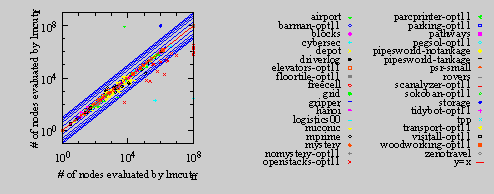
\includegraphics{tables/aaai16-5min/aaai16prelim3/evaluated-lmcut_ff-lmcut_lf.pdf}
 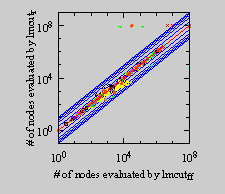
\includegraphics{tables/aaai16-5min/aaai16prelim3/evaluated-nokey-lmcut_ff-lmcut_r.pdf}
 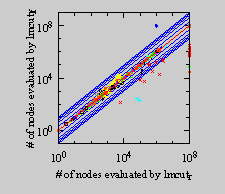
\includegraphics{tables/aaai16-5min/aaai16prelim3/evaluated-nokey-lmcut_r-lmcut_lf.pdf}
 \caption{Comparisons of \# of Evaluations between simple \lifo, \fifo,
 \ro second-level tiebreaking, with first-level $h$-tiebreaking. Each
 line shows $\times 2,4,6\ldots$ boundary.}  \label{f-h-eval}
\end{figure}

According to \reftbl{single-coverage} (left) with $h$-tiebreaking, LIFO
outperforms the other strategies, while  in Openstacks, but Random outperforms the others in
Cybersec, and FIFO performed best in Airport, and
\refig{f-h-eval} shows that Random performs best in Miconic.
\refig{f-h-eval} also shows that the difference in number of nodes evaluated can sometimes be larger than a factor of 10,
especially in Openstacks and Cybersec.
Although LIFO second-level tie-breaking appears to perform best overall on these benchmarks, 
there are no dominance relationship between these three strategies, and the overall performance of each strategy will depend on the composition of problem instances in the benchmark set.
%These differences are purely due to the domain characteristics. 

\subsection{Is $h$-Based Tie-Breaking necessary?}

Next, we investigated whether $h$-based, first-level tie-breaking is necessary.
In \reftbl{single-coverage} (right), which shows the results when  first-level
tiebreaking based on $h$ is disabled, [f, \lifo], which simply breaks ties among nodes with the same $f$-cost by expanding most recently generated nodes first (first suggested in \cite{korf85depth}),
clearly dominates [f, \fifo] and [f, \ro].

Interestingly, the performance of the [f, \lifo] strategy
is comparable to [f,h,\lifo],[f,h,\fifo], and [f,h,\ro], the two-level strategies that first break ties according to $h$.
This is somewhat surprising, considering the ubiquity of $h$-based tie-breaking in the search and planning communities.
\todo{Explanation of why [f,\lifo] performs so well. }

We reemphasize that, although LIFO dominated the others, we consider
this is just by a coincidence due to the selection of time limit, memory
limit and problems in the current standard IPC competition
settings. \emph{We are not trying to claim that any of LIFO or FIFO or
Random order always dominates the others}.

% However, there are noticeable
% performance difference caused by these different tiebreaking strategies.

\subsection{Plateaus and Tie-Breaking}

In our comparison of the simple two-level tie-breaking strategies
above, we observed that large differences in performance between
two-level tie-breaking strategies tend to occur in problems where
there are many nodes that have the same $f$ and $h$ values, creating
large \emph{plateau} regions where the heuristic does not provide
useful guidance -- in effect, these plateau regions in the last
frontier ($f=f^*$) by definition requires blind search, i.e., 
relying solely on the tie-breaking criterion, in order to escape the
plateau and find a goal node.
%, i.e., the problems where the
%heuristic function is not informative and the planner relies heavily on
%the tiebreaking criteria.

\refig{plateau} plots the size of the final search plateau on 1104 IPC benchmark instances.
The $y$-axis
represents the number of nodes with $[f,h]=[f^*,0]$, and the $x$-axis represents the total
number of nodes with $f\leq f^*$ 
Clearly, in some domains such as Openstacks and Cybersec, the planner can spend most of the runtime
searching the final plateau.
It also
means that these domains have very large variance in the runtime caused
by the difference in second-level tiebreakings. 

\refig{fig:plateau-noh} in the introduction is the same figure without $h$-tiebreaking.
Besides, as expected, when the
$h$-based tiebreaking is disabled in \refig{fig:plateau-noh}, much
larger effort could be spent on the final plateau.





%  The size of the bucket does not change
% between $[f,h,\fifo]$, $[f,h,\lifo]$ and $[f,h,\ro]$.


\begin{figure}[htb]
 \centering \relsize{-3}
  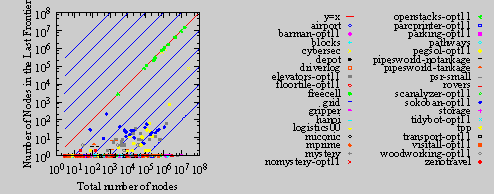
\includegraphics{tables/aaai16-frontier/aaai16prelim3/lmcut_frontier-front.pdf}
  \caption{Comparing the size of the $[f,h]$ search plateau to the total
  evaluation below $f\leq f^*$. Data were obtained by the result of
  \lmcut on the standard benchmark instances. Both axes are
  logarithmic. Dotted lines represent $\times 10^n$ boundaries.
  Openstacks clearly has the large plateaus.}  \label{plateau}
\end{figure}

\todo[Move this after zerocost domains are defined?]{}
\todo[When we plot the same statistics on the zerocost domains, this
becomes a universal trend among instances.]{Current figure is not
plotting the zerocost domains} In cost-minimization problems, the search
strategy within plateau becomes much more important than in the
runtime-minimization instances, where most actions have nonzero cost.

\begin{figure}[htb]
 \centering \relsize{-3}
  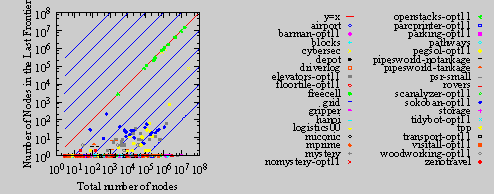
\includegraphics{tables/aaai16-frontier/aaai16prelim3/lmcut_frontier-front.pdf}
  \caption{Same plot as \refig{plateau}, but from the zerocost
  domains. Even with $h$-tiebreaking, zerocost domains force the planner
  to search much larger plateau.}
 \label{plateau-zerocost}
\end{figure}

\section{Domains with Zero-cost Actions: Applications and Motivation}
\todo{struggling to find the right place for this..}

% XXX I'm commenting out the paragraphs below because:
% (1) A review of heuristic functions for domain-independent learning is not really
% necessary for this AAAI submission. 
% (2) It's better if this paper is not so strongly associated with the ICAPS community only -- this work applies in general to search with A*, and is not strongly tied to almost-perfect heuristics, lmcut, m&s, etc.

Historically, the study of the shortest path finding algorithms has
started on the unit cost domains as the simplest case, where every
search edge has a cost 1,
% . Experimental study of \astar was somewhat biased to
% the unit-cost domains
such as 24-puzzle, Rubik's Cube etc.
There are also several problems with non-unit costs, sometimes
artificially but also sometimes naturally, such as in multiple
sequence alignment (MSA).

In the plannning community, actions with non-unit costs were first introduced in 
IPC-2002. Currently most competition domains have non-unit action costs.
Notably, most actions in these domains have nonzero positive costs.
% 
%  Although some of these domains have non-unit costs,
% those domains are sometimes \emph{mostly} unit cost. For example, TPP
% has many actions with a cost 1 and some actions have cost 10.
% 
% The idea here is to differentiate the important actions from the less
% important actions.
% 
For example, Elevator and Miconic in the benchmark domains minimize the
runtime of moving the passengers up and down.  Actions in which the
elevator travels the long distance take longer runtime.  When concerned
with the runtime, it is reasonable to assign nonzero positive cost to
every actions, since every actions are supposed to at least consume a
fraction of time.

However, such formulation is not suitable for the general type of cost
minimization in which the target is not the runtime.  For example, when
you try to minimize the energy consumption by the elevators, many
actions would have zero-cost --- it does not consume electricity for
either moving the elevator down, boarding or leaving the passenger.
 
The same thing applies to the transportation-type and assembly-type
domains like logistics and Woodworking, respectively. They are runtime
minimization domains in which driving and manual labor, or cutting and
painting, are equally measured by the single runtime metric.
% 
However, a few modifications to the action costs will turn them into
cost-minimization domains, in which the target is the fuel consumption
(logistics) or wood usage (Woodworking). From the practical point of
view, cost minimization domains would have wider interests compared to
the simple runtime minimization.

The Openstacks domain is a cost
minimization domain first introduced in IPC-2006, where the objective is to 
minimizing the number of stacks used.
There are many zero-cost actions (i.e., actions that don't increase the number of stacks), and
these zero-cost actions prevent the commonly used heuristics from producing
informative guidance, confounding commonly used heuristics.
For example, \lmcut \cite{Helmert2009} fails to find a good cost
partitioning with non-zero values, and most edges in the abstraction
space of M\&S have zero costs \cite{helmert2007flexible}.

% Currently, most benchmark domains except Openstacks and Cybersec do not
% have the large plateau thanks to the powerful heuristic estimates (which
% is verified in the later section). However, limiting our effective
% experiments only to 2 domains would bias our observation. To avoid this
% issue, we created several domains where the \sota heuristic functions
% fail to provide a menaingful guidance.

% One important characteristics shared by Openstacks and Cybersec is that they both
% have large number of zero-cost actions.
 % In such situations, both LMcut
% and M\&S fail to find a meaningful heuristic estimate because LMcut fails to
% find a good cost partitioning with non-zero values, and most edges in the abstraction space of
% M\&S have zero costs.

% We therefore modified various domains to have many zero-cost actions.
% For example, miconic-up is a domain which minimizes the energy
% consumption caused by ``up'' action, which moves the elevator up, and
% all other actions have zero-cost. Another example is driverlog-fuel, where only
% the ``drive'' action has cost 1 and all other actions are zero-cost.
% This in fact reflects the practical application compared to the original
% unit-cost domains where driving and manual labor is equally accounted.
% Oddly, although some planners have options which treats actions as if
% they are unit-costs, and describe such options as ``inadmissible'',
% solving domains which are unit-cost by origin is not called
% ``inadmissible''. Above modification addresses this problem.

In this paper, we therefore modified various domains to have many
zero-cost actions.  For example, miconic-up is a domain which minimizes
the energy consumption caused by ``up'' action, which moves the elevator
up, and all other actions have zero-cost.  Modification was done in a
practically reasonable manner in a sense of cost minimization. Most
transportation-type domains are modified so that they use less
fuel. Assembly-type domains are modified so that it minimizes the
resource usage such as ink or wood.  \todo[We also modify a same domain
in the different minimization criteria, in order to avoid the bias on a
particular domain formulation.]{It's not tested yet}





\section{Depth-based Tiebreaking}

In order to solve problems with large final plateaus, the
planner needs to run an efficient knowledge-free search within the
plateau.  One useful metric which can be used to control the search in this
situation is the \emph{depth} of a node, which represents the number 
of steps a node is from the entrance of the plateau.
$Depth(n)$ is defined as $depth(parent(n)) + 1$
If the $parent(n)$ is from the other plateau, i.e., $parent(n)$ has a different $f$-value, or different $h$-value used for the first
tiebreaking, the $depth(n) = 0$. 
Based on this simple notion of depth,
we propose  \emph{depth-based tie-breaking}, where all nodes are associated with its depth, 
and depth is used as a tie-breaking criterion.
FirstDepth(FD), RandomDepth(RD) and LastDepth(LD) breaks ties by choosing a node from 
nodes with the smallest depth ,a random depth, or the largest depth, respectively.

In the rest of thie paper, depth-based tie-breaking is used as a second-level tie-breaking criterion,
where the first tie-breaking criterion is $h$.
Since there can be multiple nodes with the same $f$, $h$ and depth,
a 3rd-level tie-breaking criterion that selects a node using FIFO, LIFO, and Random Order (R) is used.
This results in 9 configurations:
[f,h,FD,FIFO], [f,h,FD,LIFO], [f,h,FD,RO], [f,h,LD,FIFO], [f,h,LI,LIFO], [f,h,D,RO], [f,h,RD,FIFO], [f,h,RD,LIFO], [f,h,RD,RO].


The effectiveness of each strategy depends on the structure of the problem instance.
In the knowledge-free search within the plateau, all nodes have the same
$f$ and $h$ values % yes, for simplicity, I'm assuming 3-level tiebreaks, ignoring no-h for the time being..
 and it is impossible to guess whether the goal is near, far
away or in a particular distance from the entrance. \todo{``entrance'' must be defined.}
In the first case,
the search should be focused around the entrance favoring the smaller
depths, and the behavior should be much like breadth-first, and it
corresponds to FirstDepth. In the second case, the planner should
greedily explore the various area of the plateau by preferring larger
depth, much like in depth-first, and corresponds to LastDepth. In the
final case where the goal node is in a particular depth, choosing the
random depth seems the safest practice. This corresponds to the case
where RandomDepth would perform better.


Also note that, the node expansion orders of [f,h,FD,FIFO] and [f,h,LD,LIFO] are
exactly the same as [f,h,FIFO] and [f,h,LIFO], respectively,
i.e., those without the depth-based
tiebreaking.  
This is because, LIFO expands the most recently evaluated\todo{evaluated or generated?}
states, which always has the largest depth, and FIFO expands the least recently
evaluated\todo{evaluated or generated?} states, which always has the smaller depth.

% This ``greediness'' is different from the normal
% sense of ``greedy search'' --- since this greediness only holds within
% the plateau, admissibility is still maintained.
 


\subsection{Evaluating Depth-based Tiebreaking}

We evaluated the nine configurations of the three-level tie-breaking strategies described above, i.e., [f,h,depthStrategy,LFR], where the first-level tie-breaking is according to $h$ (break ties in favor of small $h$), the second-level strategy is based on depth and $depthStrategy \in \{\fd, \ld, \rd\}$, and the third level tie-breaking strategy $LFR \in \{\lifo, \fifo, \ro\}$.

In addition to the 28 standard IPC benchmark domains used in the previous set of experiments, we also added 16 \emph{zerocost} domains with 640 problems. 

Note that, the node evaluation order of $[\cdot,\fd,\fifo]$ and $[\cdot,\ld,\lifo]$
are exactly the same as those without the second-level
depth-based tiebreaking, i.e.\ $[\cdot,\fifo]$ and $[\cdot,\lifo]$.
Yet these results are useful in assessing the extra cost of managing the
depth-based buckets.

\refig{depth} shows various experiments on benchmark domains and
zerocost domains. Regardless of the third-level tiebreaking, LastDepth
strategy tends to be dominant in most domains. However, RandomDepth and
FirstDepth still exhibits a significantly better performance in Cybersec
and Mistery-Feast, respectively, indicating there is no true dominance relationship.

This result explains why the simple $[f,h,\lifo]$ strategy has become
successful. $[f,h,\lifo]$ is same as $[f,h,\ld,\lifo]$, and the fact
that the performance of $[f,h,\ld,\cdot]$ was consistently good
regardless of the third-level tiebreaking means that the performance of
$[f,h,\ld,\lifo]$ was caused by LastDepth and not by third-level LIFO tiebreaking.

Supporting the above claim, the overall dominant third-level tiebreaking
in these experiments is FIFO.  For example, when we fix the second-level
tiebreaking, the coverages are $[f,h,X,\fifo]>[f,h,X,\ro]>[f,h,X,\lifo]$
when $X=\ld,\rd$.  Note that FIFO is bad in terms of low-level memory
access pattern since the insertion and deletion happens in the opposite
side of the bucket.  This difference in the third-level tiebreaking is
more likely due to the specific action ordering in the domain
definition.  For example, in Pipesworld-Pushend, the dominant
third-level strategy is RandomOrder, regardless of the second-level
depth tiebreaking.  (FIFO,RO,LIFO is 3,3,3 in FirstDepth, 3,4,3 in
RandomDepth, and 5,6,4 in LastDepth.) Also, in $[f,h,\rd,\cdot]$, the
RandomOrder third-level tiebreaking is better than \lifo or \fifo, in
Airport-Fuel and Mprime-Succumb.

%% following discource may not be a good way to defend our paper.
% Keen readers might be concerned with the effect of action ordering in
% the domain definition. Although we showed that tie-breaking makes a
% difference, all the minor differences could be accidental and due to the
% input ordering, i.e., tiebreaking could change their behavior in some
% cases by changing the sort order of the actions.
% 
% This consideration does not diminish our depth-based second tiebreaking.
% First, the only part affected by the action ordering is the
% third tiebreaking, for which we tested \lifo, \fifo and \ro.
% We are not trying to claim some dominance relationships within these
% third tiebreakings. The purpose of the comparison 

% also, even with 2-level tiebreaking,  2nd level random tiebreaking, lmcut(f,r), did not perform that well, so that supports the claim that re-ordering alone cannot explain all the results, and lmcut(f,h,r) is significantly worse than lmcut(f,h,lifo).

% Another issue in this result is the lack of analysis on
% abstraction-based heuristics. We also added the results in the figures
% in the supplemental materials. Above trends are mostly consistent when
% M\&S and blind heuristics are used, regardless of first-level
% tiebreaking by $h$-value. However, we note that many instances quickly
% exhausted the 2GB memory limit with those heuristics, and is less
% informative compared to the result by LMcut.

\begin{figure}[htb]
 \centering
 \relsize{-3}
 \begin{tabular}{|c|c|c|c|c|c|c|c|c|c||c|c|c|c|c|c|c|c|c|}
\hline                                                      
 Domain & \rotatebox[origin=l]{90}{${\mbox{lmcut}}_{\mbox{${\mbox{fd}}_{\mbox{fifo}}$}}$}   & \rotatebox[origin=l]{90}{${\mbox{lmcut}}_{\mbox{${\mbox{rd}}_{\mbox{fifo}}$}}$}   & \rotatebox[origin=l]{90}{${\mbox{lmcut}}_{\mbox{${\mbox{ld}}_{\mbox{fifo}}$}}$}   & \rotatebox[origin=l]{90}{${\mbox{lmcut}}_{\mbox{${\mbox{fd}}_{\mbox{random}}$}}$}   & \rotatebox[origin=l]{90}{${\mbox{lmcut}}_{\mbox{${\mbox{rd}}_{\mbox{random}}$}}$}   & \rotatebox[origin=l]{90}{${\mbox{lmcut}}_{\mbox{${\mbox{ld}}_{\mbox{random}}$}}$}   & \rotatebox[origin=l]{90}{${\mbox{lmcut}}_{\mbox{${\mbox{fd}}_{\mbox{lifo}}$}}$}   & \rotatebox[origin=l]{90}{${\mbox{lmcut}}_{\mbox{${\mbox{rd}}_{\mbox{lifo}}$}}$}   & \rotatebox[origin=l]{90}{${\mbox{lmcut}}_{\mbox{${\mbox{ld}}_{\mbox{lifo}}$}}$}   & \rotatebox[origin=l]{90}{${\mbox{mands}}_{\mbox{${\mbox{fd}}_{\mbox{fifo}}$}}$}   & \rotatebox[origin=l]{90}{${\mbox{mands}}_{\mbox{${\mbox{rd}}_{\mbox{fifo}}$}}$}   & \rotatebox[origin=l]{90}{${\mbox{mands}}_{\mbox{${\mbox{ld}}_{\mbox{fifo}}$}}$}   & \rotatebox[origin=l]{90}{${\mbox{mands}}_{\mbox{${\mbox{fd}}_{\mbox{random}}$}}$}   & \rotatebox[origin=l]{90}{${\mbox{mands}}_{\mbox{${\mbox{rd}}_{\mbox{random}}$}}$}   & \rotatebox[origin=l]{90}{${\mbox{mands}}_{\mbox{${\mbox{ld}}_{\mbox{random}}$}}$}   & \rotatebox[origin=l]{90}{${\mbox{mands}}_{\mbox{${\mbox{fd}}_{\mbox{lifo}}$}}$}   & \rotatebox[origin=l]{90}{${\mbox{mands}}_{\mbox{${\mbox{rd}}_{\mbox{lifo}}$}}$}   & \rotatebox[origin=l]{90}{${\mbox{mands}}_{\mbox{${\mbox{ld}}_{\mbox{lifo}}$}}$}    \\
\hline                                                      
 sum(1104) &  558 &  \textbf{568} &  \textbf{568} &  556 &  565 &  565 &  558 &  567 &  565 &  484 &  489 &  490 &  471 &  479 &  481 &  484 &  489 &  490  \\
\hline                                                      
 {\relsize{-1}airport(50)} &  \textbf{27} &  \textbf{27} &  \textbf{27} &  25 &  25 &  25 &  26 &  26 &  26 &  9 &  9 &  9 &  9 &  9 &  9 &  9 &  9 &  9  \\
 {\relsize{-1}barman-opt11(20)} &  0 &  0 &  0 &  0 &  0 &  0 &  0 &  0 &  0 &  \textbf{4} &  \textbf{4} &  \textbf{4} &  \textbf{4} &  \textbf{4} &  \textbf{4} &  \textbf{4} &  \textbf{4} &  \textbf{4}  \\
 {\relsize{-1}blocks(35)} &  \textbf{28} &  \textbf{28} &  \textbf{28} &  \textbf{28} &  \textbf{28} &  \textbf{28} &  \textbf{28} &  \textbf{28} &  \textbf{28} &  22 &  22 &  22 &  22 &  22 &  22 &  21 &  21 &  21  \\
 {\relsize{-1}cybersec(19)} &  1 &  \textbf{3} &  \textbf{3} &  2 &  \textbf{3} &  \textbf{3} &  2 &  \textbf{3} &  2 &  0 &  0 &  0 &  0 &  0 &  0 &  0 &  0 &  0  \\
 {\relsize{-1}depot(22)} &  \textbf{6} &  \textbf{6} &  \textbf{6} &  \textbf{6} &  \textbf{6} &  \textbf{6} &  \textbf{6} &  \textbf{6} &  \textbf{6} &  \textbf{6} &  \textbf{6} &  \textbf{6} &  5 &  5 &  5 &  \textbf{6} &  \textbf{6} &  \textbf{6}  \\
 {\relsize{-1}driverlog(20)} &  \textbf{13} &  \textbf{13} &  \textbf{13} &  \textbf{13} &  \textbf{13} &  \textbf{13} &  \textbf{13} &  \textbf{13} &  \textbf{13} &  12 &  12 &  12 &  12 &  12 &  12 &  12 &  12 &  12  \\
 {\relsize{-1}elevators-opt11(20)} &  \textbf{15} &  \textbf{15} &  \textbf{15} &  \textbf{15} &  \textbf{15} &  \textbf{15} &  \textbf{15} &  \textbf{15} &  \textbf{15} &  12 &  12 &  12 &  12 &  12 &  12 &  12 &  12 &  12  \\
 {\relsize{-1}freecell(80)} &  9 &  9 &  9 &  9 &  9 &  9 &  9 &  9 &  9 &  \textbf{17} &  \textbf{17} &  \textbf{17} &  15 &  15 &  15 &  \textbf{17} &  \textbf{17} &  \textbf{17}  \\
 {\relsize{-1}grid(5)} &  1 &  1 &  1 &  1 &  1 &  1 &  1 &  1 &  1 &  \textbf{2} &  \textbf{2} &  \textbf{2} &  \textbf{2} &  \textbf{2} &  \textbf{2} &  \textbf{2} &  \textbf{2} &  \textbf{2}  \\
 {\relsize{-1}gripper(20)} &  6 &  6 &  6 &  6 &  6 &  6 &  6 &  6 &  6 &  \textbf{20} &  \textbf{20} &  \textbf{20} &  \textbf{20} &  \textbf{20} &  \textbf{20} &  \textbf{20} &  \textbf{20} &  \textbf{20}  \\
 {\relsize{-1}hanoi(30)} &  12 &  12 &  12 &  12 &  12 &  12 &  12 &  12 &  12 &  \textbf{14} &  \textbf{14} &  \textbf{14} &  \textbf{14} &  \textbf{14} &  \textbf{14} &  \textbf{14} &  \textbf{14} &  \textbf{14}  \\
 {\relsize{-1}miconic(150)} &  \textbf{140} &  \textbf{140} &  \textbf{140} &  \textbf{140} &  \textbf{140} &  \textbf{140} &  \textbf{140} &  \textbf{140} &  \textbf{140} &  73 &  73 &  73 &  72 &  72 &  72 &  73 &  73 &  73  \\
 {\relsize{-1}mprime(35)} &  21 &  21 &  21 &  21 &  21 &  21 &  21 &  21 &  21 &  23 &  23 &  23 &  23 &  23 &  23 &  \textbf{24} &  \textbf{24} &  \textbf{24}  \\
 {\relsize{-1}mystery(30)} &  15 &  \textbf{16} &  \textbf{16} &  15 &  15 &  15 &  \textbf{16} &  \textbf{16} &  15 &  15 &  15 &  15 &  15 &  15 &  15 &  \textbf{16} &  \textbf{16} &  \textbf{16}  \\
 {\relsize{-1}nomystery-opt11(20)} &  14 &  14 &  14 &  14 &  14 &  14 &  14 &  14 &  14 &  \textbf{18} &  \textbf{18} &  \textbf{18} &  \textbf{18} &  \textbf{18} &  \textbf{18} &  \textbf{18} &  \textbf{18} &  \textbf{18}  \\
 {\relsize{-1}openstacks-opt11(20)} &  12 &  18 &  18 &  10 &  18 &  18 &  11 &  18 &  18 &  13 &  \textbf{19} &  \textbf{19} &  9 &  18 &  \textbf{19} &  13 &  \textbf{19} &  \textbf{19}  \\
 {\relsize{-1}parcprinter-opt11(20)} &  \textbf{13} &  \textbf{13} &  \textbf{13} &  \textbf{13} &  \textbf{13} &  \textbf{13} &  \textbf{13} &  \textbf{13} &  \textbf{13} &  10 &  9 &  10 &  10 &  9 &  10 &  10 &  9 &  10  \\
 {\relsize{-1}pathways(30)} &  \textbf{5} &  \textbf{5} &  \textbf{5} &  \textbf{5} &  \textbf{5} &  \textbf{5} &  \textbf{5} &  \textbf{5} &  \textbf{5} &  4 &  4 &  4 &  4 &  4 &  4 &  4 &  4 &  4  \\
 {\relsize{-1}pegsol-opt11(20)} &  17 &  17 &  17 &  17 &  17 &  17 &  17 &  17 &  17 &  \textbf{19} &  \textbf{19} &  \textbf{19} &  18 &  18 &  18 &  \textbf{19} &  \textbf{19} &  \textbf{19}  \\
 {\relsize{-1}pipesworld-notankage(50)} &  \textbf{15} &  \textbf{15} &  \textbf{15} &  \textbf{15} &  \textbf{15} &  \textbf{15} &  \textbf{15} &  \textbf{15} &  \textbf{15} &  10 &  10 &  10 &  9 &  9 &  9 &  9 &  9 &  9  \\
 {\relsize{-1}pipesworld-tankage(50)} &  8 &  8 &  8 &  8 &  8 &  8 &  8 &  8 &  8 &  \textbf{13} &  \textbf{13} &  \textbf{13} &  12 &  12 &  12 &  \textbf{13} &  \textbf{13} &  \textbf{13}  \\
 {\relsize{-1}psr-small(50)} &  48 &  48 &  48 &  48 &  48 &  48 &  48 &  48 &  48 &  \textbf{50} &  \textbf{50} &  \textbf{50} &  \textbf{50} &  \textbf{50} &  \textbf{50} &  \textbf{50} &  \textbf{50} &  \textbf{50}  \\
 {\relsize{-1}rovers(40)} &  7 &  7 &  7 &  7 &  7 &  7 &  7 &  7 &  7 &  \textbf{8} &  \textbf{8} &  \textbf{8} &  6 &  6 &  6 &  \textbf{8} &  \textbf{8} &  \textbf{8}  \\
 {\relsize{-1}sokoban-opt11(20)} &  19 &  19 &  19 &  19 &  19 &  19 &  19 &  19 &  19 &  \textbf{20} &  \textbf{20} &  \textbf{20} &  \textbf{20} &  \textbf{20} &  \textbf{20} &  \textbf{20} &  \textbf{20} &  \textbf{20}  \\
 {\relsize{-1}storage(30)} &  \textbf{15} &  \textbf{15} &  \textbf{15} &  \textbf{15} &  \textbf{15} &  \textbf{15} &  14 &  \textbf{15} &  \textbf{15} &  \textbf{15} &  \textbf{15} &  \textbf{15} &  \textbf{15} &  \textbf{15} &  \textbf{15} &  \textbf{15} &  \textbf{15} &  \textbf{15}  \\
 {\relsize{-1}tidybot-opt11(20)} &  \textbf{12} &  \textbf{12} &  \textbf{12} &  \textbf{12} &  \textbf{12} &  \textbf{12} &  \textbf{12} &  \textbf{12} &  \textbf{12} &  0 &  0 &  0 &  0 &  0 &  0 &  0 &  0 &  0  \\
 {\relsize{-1}visitall-opt11(20)} &  \textbf{10} &  \textbf{10} &  \textbf{10} &  \textbf{10} &  \textbf{10} &  \textbf{10} &  \textbf{10} &  \textbf{10} &  \textbf{10} &  9 &  9 &  9 &  9 &  9 &  9 &  9 &  9 &  9  \\
 {\relsize{-1}woodworking-opt11(20)} &  \textbf{10} &  \textbf{10} &  \textbf{10} &  \textbf{10} &  \textbf{10} &  \textbf{10} &  \textbf{10} &  \textbf{10} &  \textbf{10} &  7 &  7 &  7 &  7 &  7 &  7 &  7 &  7 &  7  \\
 {\relsize{-1}zenotravel(20)} &  10 &  \textbf{11} &  \textbf{11} &  \textbf{11} &  \textbf{11} &  \textbf{11} &  \textbf{11} &  \textbf{11} &  \textbf{11} &  10 &  10 &  10 &  10 &  10 &  10 &  10 &  10 &  10 \\
\hline
 sum(380) &  163 &  175 &  \textbf{177} &  158 &  172 &  173 &  164 &  167 &  165 &  169 &  176 &  176 &  161 &  173 &  171 &  168 &  167 &  165  \\
\hline                                                      
 {\relsize{-1}airport-fuel(20)} &  \textbf{15} &  14 &  14 &  14 &  13 &  13 &  14 &  \textbf{15} &  14 &  5 &  5 &  5 &  5 &  5 &  5 &  5 &  5 &  5  \\
 {\relsize{-1}depot-fuel(22)} &  \textbf{6} &  \textbf{6} &  \textbf{6} &  \textbf{6} &  \textbf{6} &  \textbf{6} &  \textbf{6} &  \textbf{6} &  \textbf{6} &  5 &  5 &  4 &  3 &  \textbf{6} &  4 &  5 &  5 &  3  \\
 {\relsize{-1}driverlog-fuel(20)} &  8 &  8 &  7 &  8 &  8 &  7 &  8 &  8 &  7 &  \textbf{9} &  \textbf{9} &  8 &  8 &  \textbf{9} &  8 &  \textbf{9} &  \textbf{9} &  8  \\
 {\relsize{-1}floortile-ink(20)} &  \textbf{8} &  \textbf{8} &  \textbf{8} &  \textbf{8} &  \textbf{8} &  \textbf{8} &  \textbf{8} &  \textbf{8} &  \textbf{8} &  7 &  7 &  7 &  6 &  7 &  7 &  6 &  7 &  6  \\
 {\relsize{-1}grid-fuel(5)} &  1 &  1 &  1 &  1 &  1 &  1 &  1 &  1 &  1 &  \textbf{2} &  \textbf{2} &  \textbf{2} &  \textbf{2} &  \textbf{2} &  \textbf{2} &  \textbf{2} &  \textbf{2} &  \textbf{2}  \\
 {\relsize{-1}hiking-fuel(20)} &  9 &  9 &  9 &  9 &  9 &  9 &  9 &  9 &  9 &  \textbf{13} &  \textbf{13} &  \textbf{13} &  11 &  11 &  11 &  \textbf{13} &  \textbf{13} &  \textbf{13}  \\
 {\relsize{-1}logistics00-fuel(28)} &  \textbf{16} &  \textbf{16} &  \textbf{16} &  15 &  15 &  15 &  \textbf{16} &  \textbf{16} &  \textbf{16} &  \textbf{16} &  \textbf{16} &  \textbf{16} &  \textbf{16} &  \textbf{16} &  \textbf{16} &  \textbf{16} &  \textbf{16} &  \textbf{16}  \\
 {\relsize{-1}miconic-up(30)} &  16 &  20 &  20 &  15 &  20 &  20 &  16 &  18 &  18 &  29 &  \textbf{30} &  \textbf{30} &  29 &  \textbf{30} &  \textbf{30} &  29 &  \textbf{30} &  \textbf{30}  \\
 {\relsize{-1}mprime-succumb(35)} &  15 &  21 &  25 &  15 &  21 &  23 &  17 &  15 &  14 &  21 &  25 &  \textbf{27} &  19 &  23 &  24 &  21 &  17 &  19  \\
 {\relsize{-1}nomystery-fuel(20)} &  10 &  10 &  10 &  10 &  10 &  10 &  10 &  10 &  10 &  \textbf{16} &  \textbf{16} &  \textbf{16} &  \textbf{16} &  \textbf{16} &  \textbf{16} &  \textbf{16} &  \textbf{16} &  \textbf{16}  \\
 {\relsize{-1}pathways-fuel(30)} &  \textbf{5} &  \textbf{5} &  4 &  4 &  4 &  4 &  \textbf{5} &  \textbf{5} &  \textbf{5} &  4 &  4 &  4 &  4 &  4 &  4 &  4 &  4 &  4  \\
 {\relsize{-1}tidybot-motion(20)} &  \textbf{16} &  \textbf{16} &  \textbf{16} &  \textbf{16} &  \textbf{16} &  \textbf{16} &  \textbf{16} &  \textbf{16} &  \textbf{16} &  0 &  0 &  0 &  0 &  0 &  0 &  0 &  0 &  0  \\
 {\relsize{-1}tpp-fuel(30)} &  8 &  \textbf{11} &  \textbf{11} &  7 &  \textbf{11} &  \textbf{11} &  8 &  10 &  \textbf{11} &  9 &  \textbf{11} &  \textbf{11} &  9 &  \textbf{11} &  \textbf{11} &  9 &  10 &  10  \\
 {\relsize{-1}zenotravel-fuel(20)} &  7 &  7 &  7 &  7 &  7 &  7 &  7 &  7 &  7 &  \textbf{10} &  \textbf{10} &  \textbf{10} &  \textbf{10} &  \textbf{10} &  \textbf{10} &  \textbf{10} &  \textbf{10} &  \textbf{10} \\
\hline
 sum(260) &  109 &  129 &  135 &  103 &  127 &  137 &  110 &  127 &  130 &  125 &  143 &  145 &  114 &  \textbf{150} &  \textbf{150} &  123 &  142 &  143  \\
\hline                                                      
 {\relsize{-1}blocks-stack(20)} &  17 &  17 &  18 &  17 &  17 &  18 &  17 &  17 &  17 &  \textbf{20} &  \textbf{20} &  \textbf{20} &  \textbf{20} &  \textbf{20} &  \textbf{20} &  \textbf{20} &  \textbf{20} &  \textbf{20}  \\
 {\relsize{-1}elevators-up(20)} &  7 &  9 &  11 &  5 &  10 &  11 &  7 &  11 &  \textbf{13} &  7 &  10 &  12 &  6 &  11 &  12 &  7 &  \textbf{13} &  \textbf{13}  \\
 {\relsize{-1}freecell-move(20)} &  4 &  16 &  \textbf{20} &  4 &  16 &  \textbf{20} &  4 &  18 &  19 &  5 &  17 &  \textbf{20} &  4 &  19 &  \textbf{20} &  5 &  14 &  19  \\
 {\relsize{-1}gripper-move(20)} &  7 &  7 &  7 &  6 &  6 &  6 &  7 &  7 &  7 &  \textbf{20} &  \textbf{20} &  \textbf{20} &  \textbf{20} &  \textbf{20} &  \textbf{20} &  \textbf{20} &  \textbf{20} &  \textbf{20}  \\
 {\relsize{-1}mystery-feast(20)} &  \textbf{8} &  7 &  6 &  7 &  7 &  6 &  \textbf{8} &  7 &  6 &  4 &  4 &  5 &  3 &  4 &  4 &  4 &  4 &  4  \\
 {\relsize{-1}pipesnt-pushstart(20)} &  8 &  \textbf{10} &  \textbf{10} &  8 &  \textbf{10} &  \textbf{10} &  8 &  8 &  8 &  3 &  5 &  5 &  3 &  5 &  5 &  3 &  3 &  3  \\
 {\relsize{-1}pipesworld-pushend(20)} &  3 &  3 &  5 &  3 &  4 &  6 &  3 &  3 &  4 &  6 &  7 &  9 &  5 &  9 &  \textbf{10} &  6 &  9 &  9  \\
 {\relsize{-1}psr-small-open(20)} &  \textbf{19} &  \textbf{19} &  \textbf{19} &  18 &  \textbf{19} &  \textbf{19} &  \textbf{19} &  \textbf{19} &  \textbf{19} &  \textbf{19} &  \textbf{19} &  \textbf{19} &  18 &  \textbf{19} &  \textbf{19} &  \textbf{19} &  \textbf{19} &  \textbf{19}  \\
 {\relsize{-1}scanalyzer-analyze(20)} &  9 &  10 &  9 &  9 &  9 &  9 &  10 &  9 &  9 &  \textbf{11} &  \textbf{11} &  9 &  10 &  \textbf{11} &  10 &  \textbf{11} &  \textbf{11} &  9  \\
 {\relsize{-1}sokoban-pushgoal(20)} &  18 &  18 &  17 &  18 &  18 &  17 &  18 &  18 &  17 &  \textbf{19} &  18 &  15 &  18 &  18 &  17 &  \textbf{19} &  18 &  16  \\
 {\relsize{-1}storage-lift(20)} &  4 &  5 &  \textbf{6} &  4 &  4 &  5 &  4 &  4 &  4 &  4 &  4 &  4 &  3 &  4 &  4 &  4 &  4 &  4  \\
 {\relsize{-1}woodworking-cut(20)} &  5 &  8 &  7 &  4 &  7 &  \textbf{10} &  5 &  6 &  7 &  7 &  8 &  7 &  4 &  \textbf{10} &  9 &  5 &  7 &  7 \\
\hline
 total(1744) &  830 &  872 &  \textbf{880} &  817 &  864 &  875 &  832 &  861 &  860 &  778 &  808 &  811 &  746 &  802 &  802 &  775 &  798 &  798 \\
\hline
\end{tabular}

 \caption{Experiments
 comparing the coverages of 9 configurations (3 depth-based strategy
 $\times$ 3 queue implementions). For the space reason, we omitted those
 domains whose results are the same. (Full results are available in the
 supplemental material.) Each cell denotes the problem solved with 30
 min, 2GB setting. \textbf{Boldface} denotes the case where it achieved
 the best result among configurations. Zerocost domains are named
 according to [original]-[name of nonzero action].}
 \label{depth}
\end{figure}

%% obviously does not fit in the paper
% \begin{figure}[htb]
%  \centering
%  \relsize{-3}
%  \begin{tabular}{|c|c|c|c|c|c|c|c|c|c||c|c|c|c|c|c|c|c|c|}
\hline                                                      
 Domain & \rotatebox[origin=l]{90}{${\mbox{lmcut}}_{\mbox{${\mbox{fd}}_{\mbox{${\mbox{fifo}}_{\mbox{noh}}$}}$}}$}   & \rotatebox[origin=l]{90}{${\mbox{lmcut}}_{\mbox{${\mbox{rd}}_{\mbox{${\mbox{fifo}}_{\mbox{noh}}$}}$}}$}   & \rotatebox[origin=l]{90}{${\mbox{lmcut}}_{\mbox{${\mbox{ld}}_{\mbox{${\mbox{fifo}}_{\mbox{noh}}$}}$}}$}   & \rotatebox[origin=l]{90}{${\mbox{lmcut}}_{\mbox{${\mbox{fd}}_{\mbox{${\mbox{random}}_{\mbox{noh}}$}}$}}$}   & \rotatebox[origin=l]{90}{${\mbox{lmcut}}_{\mbox{${\mbox{rd}}_{\mbox{${\mbox{random}}_{\mbox{noh}}$}}$}}$}   & \rotatebox[origin=l]{90}{${\mbox{lmcut}}_{\mbox{${\mbox{ld}}_{\mbox{${\mbox{random}}_{\mbox{noh}}$}}$}}$}   & \rotatebox[origin=l]{90}{${\mbox{lmcut}}_{\mbox{${\mbox{fd}}_{\mbox{${\mbox{lifo}}_{\mbox{noh}}$}}$}}$}   & \rotatebox[origin=l]{90}{${\mbox{lmcut}}_{\mbox{${\mbox{rd}}_{\mbox{${\mbox{lifo}}_{\mbox{noh}}$}}$}}$}   & \rotatebox[origin=l]{90}{${\mbox{lmcut}}_{\mbox{${\mbox{ld}}_{\mbox{${\mbox{lifo}}_{\mbox{noh}}$}}$}}$}   & \rotatebox[origin=l]{90}{${\mbox{mands}}_{\mbox{${\mbox{fd}}_{\mbox{${\mbox{fifo}}_{\mbox{noh}}$}}$}}$}   & \rotatebox[origin=l]{90}{${\mbox{mands}}_{\mbox{${\mbox{rd}}_{\mbox{${\mbox{fifo}}_{\mbox{noh}}$}}$}}$}   & \rotatebox[origin=l]{90}{${\mbox{mands}}_{\mbox{${\mbox{ld}}_{\mbox{${\mbox{fifo}}_{\mbox{noh}}$}}$}}$}   & \rotatebox[origin=l]{90}{${\mbox{mands}}_{\mbox{${\mbox{fd}}_{\mbox{${\mbox{random}}_{\mbox{noh}}$}}$}}$}   & \rotatebox[origin=l]{90}{${\mbox{mands}}_{\mbox{${\mbox{rd}}_{\mbox{${\mbox{random}}_{\mbox{noh}}$}}$}}$}   & \rotatebox[origin=l]{90}{${\mbox{mands}}_{\mbox{${\mbox{ld}}_{\mbox{${\mbox{random}}_{\mbox{noh}}$}}$}}$}   & \rotatebox[origin=l]{90}{${\mbox{mands}}_{\mbox{${\mbox{fd}}_{\mbox{${\mbox{lifo}}_{\mbox{noh}}$}}$}}$}   & \rotatebox[origin=l]{90}{${\mbox{mands}}_{\mbox{${\mbox{rd}}_{\mbox{${\mbox{lifo}}_{\mbox{noh}}$}}$}}$}   & \rotatebox[origin=l]{90}{${\mbox{mands}}_{\mbox{${\mbox{ld}}_{\mbox{${\mbox{lifo}}_{\mbox{noh}}$}}$}}$}    \\
\hline                                                      
 sum(1104) &  446 &  538 &  559 &  441 &  \textbf{564} &  \textbf{564} &  445 &  545 &  560 &  452 &  482 &  482 &  424 &  461 &  464 &  453 &  486 &  484  \\
\hline                                                      
 {\relsize{-1}airport(50)} &  18 &  21 &  25 &  18 &  21 &  \textbf{26} &  18 &  22 &  25 &  9 &  9 &  9 &  9 &  9 &  9 &  9 &  9 &  9  \\
 {\relsize{-1}barman-opt11(20)} &  0 &  0 &  0 &  0 &  0 &  0 &  0 &  0 &  0 &  \textbf{4} &  \textbf{4} &  \textbf{4} &  \textbf{4} &  \textbf{4} &  \textbf{4} &  \textbf{4} &  \textbf{4} &  \textbf{4}  \\
 {\relsize{-1}blocks(35)} &  26 &  \textbf{28} &  \textbf{28} &  26 &  \textbf{28} &  26 &  26 &  27 &  27 &  21 &  21 &  21 &  19 &  19 &  20 &  21 &  21 &  21  \\
 {\relsize{-1}cybersec(19)} &  0 &  2 &  3 &  0 &  \textbf{4} &  \textbf{4} &  0 &  \textbf{4} &  2 &  0 &  0 &  0 &  0 &  0 &  0 &  0 &  0 &  0  \\
 {\relsize{-1}depot(22)} &  5 &  \textbf{6} &  \textbf{6} &  5 &  \textbf{6} &  \textbf{6} &  5 &  \textbf{6} &  \textbf{6} &  5 &  5 &  \textbf{6} &  4 &  5 &  5 &  5 &  \textbf{6} &  \textbf{6}  \\
 {\relsize{-1}driverlog(20)} &  12 &  12 &  12 &  12 &  \textbf{13} &  \textbf{13} &  12 &  \textbf{13} &  \textbf{13} &  11 &  12 &  12 &  11 &  11 &  11 &  11 &  12 &  12  \\
 {\relsize{-1}elevators-opt11(20)} &  14 &  14 &  14 &  14 &  \textbf{15} &  \textbf{15} &  14 &  \textbf{15} &  \textbf{15} &  11 &  11 &  11 &  10 &  11 &  11 &  11 &  11 &  11  \\
 {\relsize{-1}floortile-opt11(20)} &  \textbf{6} &  \textbf{6} &  \textbf{6} &  \textbf{6} &  \textbf{6} &  \textbf{6} &  \textbf{6} &  \textbf{6} &  \textbf{6} &  5 &  5 &  5 &  4 &  4 &  4 &  5 &  5 &  5  \\
 {\relsize{-1}freecell(80)} &  9 &  9 &  9 &  8 &  9 &  9 &  8 &  9 &  9 &  15 &  \textbf{16} &  \textbf{16} &  14 &  14 &  14 &  15 &  \textbf{16} &  \textbf{16}  \\
 {\relsize{-1}grid(5)} &  1 &  1 &  1 &  1 &  1 &  1 &  1 &  1 &  1 &  \textbf{2} &  \textbf{2} &  \textbf{2} &  \textbf{2} &  \textbf{2} &  \textbf{2} &  \textbf{2} &  \textbf{2} &  \textbf{2}  \\
 {\relsize{-1}gripper(20)} &  6 &  6 &  6 &  6 &  6 &  6 &  6 &  6 &  6 &  7 &  \textbf{20} &  \textbf{20} &  6 &  \textbf{20} &  \textbf{20} &  7 &  \textbf{20} &  \textbf{20}  \\
 {\relsize{-1}hanoi(30)} &  12 &  12 &  12 &  12 &  12 &  12 &  12 &  12 &  12 &  \textbf{14} &  \textbf{14} &  \textbf{14} &  \textbf{14} &  \textbf{14} &  \textbf{14} &  \textbf{14} &  \textbf{14} &  \textbf{14}  \\
 {\relsize{-1}logistics00(28)} &  16 &  \textbf{20} &  \textbf{20} &  16 &  \textbf{20} &  \textbf{20} &  16 &  19 &  19 &  \textbf{20} &  \textbf{20} &  \textbf{20} &  17 &  19 &  19 &  \textbf{20} &  \textbf{20} &  \textbf{20}  \\
 {\relsize{-1}miconic(150)} &  68 &  126 &  \textbf{140} &  68 &  \textbf{140} &  \textbf{140} &  68 &  125 &  \textbf{140} &  68 &  72 &  72 &  68 &  70 &  70 &  68 &  73 &  72  \\
 {\relsize{-1}mprime(35)} &  20 &  22 &  22 &  20 &  21 &  21 &  20 &  22 &  22 &  \textbf{23} &  \textbf{23} &  \textbf{23} &  22 &  22 &  \textbf{23} &  \textbf{23} &  \textbf{23} &  \textbf{23}  \\
 {\relsize{-1}mystery(30)} &  15 &  \textbf{16} &  \textbf{16} &  15 &  \textbf{16} &  \textbf{16} &  15 &  \textbf{16} &  \textbf{16} &  15 &  15 &  15 &  15 &  15 &  15 &  15 &  15 &  15  \\
 {\relsize{-1}nomystery-opt11(20)} &  12 &  12 &  12 &  12 &  14 &  14 &  12 &  13 &  14 &  17 &  \textbf{18} &  \textbf{18} &  16 &  \textbf{18} &  \textbf{18} &  17 &  \textbf{18} &  \textbf{18}  \\
 {\relsize{-1}openstacks-opt11(20)} &  12 &  18 &  18 &  10 &  18 &  18 &  12 &  18 &  18 &  13 &  \textbf{19} &  \textbf{19} &  9 &  18 &  \textbf{19} &  13 &  \textbf{19} &  \textbf{19}  \\
 {\relsize{-1}parcprinter-opt11(20)} &  12 &  \textbf{13} &  \textbf{13} &  12 &  \textbf{13} &  \textbf{13} &  12 &  \textbf{13} &  \textbf{13} &  10 &  10 &  10 &  10 &  10 &  10 &  10 &  10 &  10  \\
 {\relsize{-1}pathways(30)} &  4 &  \textbf{5} &  \textbf{5} &  4 &  \textbf{5} &  \textbf{5} &  4 &  \textbf{5} &  \textbf{5} &  4 &  4 &  4 &  4 &  4 &  4 &  4 &  4 &  4  \\
 {\relsize{-1}pegsol-opt11(20)} &  17 &  17 &  17 &  16 &  17 &  17 &  17 &  17 &  17 &  17 &  17 &  17 &  16 &  17 &  17 &  17 &  \textbf{19} &  \textbf{19}  \\
 {\relsize{-1}pipesworld-notankage(50)} &  13 &  13 &  13 &  13 &  \textbf{15} &  \textbf{15} &  13 &  13 &  13 &  8 &  10 &  9 &  8 &  8 &  8 &  9 &  10 &  9  \\
 {\relsize{-1}pipesworld-tankage(50)} &  7 &  8 &  8 &  7 &  8 &  8 &  7 &  8 &  8 &  \textbf{13} &  \textbf{13} &  \textbf{13} &  12 &  12 &  12 &  \textbf{13} &  \textbf{13} &  \textbf{13}  \\
 {\relsize{-1}psr-small(50)} &  48 &  48 &  48 &  48 &  48 &  48 &  48 &  48 &  48 &  \textbf{50} &  \textbf{50} &  \textbf{50} &  48 &  48 &  48 &  \textbf{50} &  \textbf{50} &  \textbf{50}  \\
 {\relsize{-1}rovers(40)} &  7 &  7 &  7 &  7 &  7 &  7 &  7 &  7 &  7 &  6 &  \textbf{8} &  \textbf{8} &  5 &  6 &  6 &  6 &  \textbf{8} &  \textbf{8}  \\
 {\relsize{-1}scanalyzer-opt11(20)} &  4 &  9 &  \textbf{10} &  4 &  9 &  \textbf{10} &  4 &  9 &  \textbf{10} &  \textbf{10} &  \textbf{10} &  \textbf{10} &  7 &  8 &  8 &  \textbf{10} &  \textbf{10} &  \textbf{10}  \\
 {\relsize{-1}sokoban-opt11(20)} &  19 &  19 &  19 &  19 &  19 &  19 &  19 &  19 &  19 &  \textbf{20} &  \textbf{20} &  \textbf{20} &  18 &  \textbf{20} &  \textbf{20} &  \textbf{20} &  \textbf{20} &  \textbf{20}  \\
 {\relsize{-1}storage(30)} &  14 &  14 &  14 &  14 &  \textbf{15} &  \textbf{15} &  14 &  14 &  14 &  \textbf{15} &  \textbf{15} &  \textbf{15} &  14 &  14 &  14 &  \textbf{15} &  \textbf{15} &  \textbf{15}  \\
 {\relsize{-1}tidybot-opt11(20)} &  11 &  11 &  11 &  11 &  \textbf{12} &  \textbf{12} &  11 &  \textbf{12} &  \textbf{12} &  0 &  0 &  0 &  0 &  0 &  0 &  0 &  0 &  0  \\
 {\relsize{-1}visitall-opt11(20)} &  \textbf{10} &  \textbf{10} &  \textbf{10} &  9 &  \textbf{10} &  \textbf{10} &  \textbf{10} &  \textbf{10} &  \textbf{10} &  9 &  9 &  9 &  9 &  9 &  9 &  9 &  9 &  9  \\
 {\relsize{-1}woodworking-opt11(20)} &  6 &  9 &  10 &  6 &  \textbf{12} &  8 &  6 &  \textbf{12} &  9 &  7 &  7 &  7 &  7 &  7 &  7 &  7 &  7 &  7  \\
 {\relsize{-1}zenotravel(20)} &  9 &  \textbf{11} &  \textbf{11} &  9 &  \textbf{11} &  \textbf{11} &  9 &  \textbf{11} &  \textbf{11} &  10 &  10 &  10 &  9 &  10 &  10 &  10 &  10 &  10 \\
\hline
 sum(380) &  137 &  165 &  172 &  133 &  169 &  170 &  139 &  164 &  166 &  143 &  173 &  \textbf{174} &  140 &  172 &  170 &  143 &  166 &  165  \\
\hline                                                      
 {\relsize{-1}airport-fuel(20)} &  7 &  10 &  14 &  8 &  10 &  14 &  8 &  12 &  \textbf{15} &  5 &  5 &  5 &  5 &  5 &  5 &  5 &  5 &  5  \\
 {\relsize{-1}depot-fuel(22)} &  5 &  \textbf{6} &  \textbf{6} &  5 &  \textbf{6} &  \textbf{6} &  5 &  \textbf{6} &  \textbf{6} &  5 &  5 &  4 &  3 &  5 &  4 &  5 &  5 &  3  \\
 {\relsize{-1}driverlog-fuel(20)} &  7 &  8 &  6 &  6 &  8 &  5 &  7 &  7 &  7 &  8 &  \textbf{9} &  8 &  8 &  \textbf{9} &  8 &  8 &  \textbf{9} &  8  \\
 {\relsize{-1}floortile-ink(20)} &  \textbf{8} &  \textbf{8} &  \textbf{8} &  \textbf{8} &  \textbf{8} &  \textbf{8} &  \textbf{8} &  \textbf{8} &  \textbf{8} &  6 &  7 &  7 &  6 &  7 &  6 &  6 &  \textbf{8} &  7  \\
 {\relsize{-1}ged-opt14(20)} &  \textbf{15} &  13 &  13 &  13 &  \textbf{15} &  14 &  \textbf{15} &  \textbf{15} &  \textbf{15} &  \textbf{15} &  \textbf{15} &  \textbf{15} &  \textbf{15} &  \textbf{15} &  \textbf{15} &  \textbf{15} &  \textbf{15} &  \textbf{15}  \\
 {\relsize{-1}grid-fuel(5)} &  1 &  1 &  1 &  1 &  1 &  1 &  1 &  1 &  1 &  \textbf{2} &  \textbf{2} &  \textbf{2} &  \textbf{2} &  \textbf{2} &  \textbf{2} &  \textbf{2} &  \textbf{2} &  \textbf{2}  \\
 {\relsize{-1}hiking-fuel(20)} &  8 &  9 &  9 &  8 &  9 &  9 &  8 &  9 &  9 &  11 &  \textbf{13} &  \textbf{13} &  10 &  11 &  11 &  11 &  \textbf{13} &  \textbf{13}  \\
 {\relsize{-1}logistics00-fuel(28)} &  15 &  \textbf{16} &  15 &  15 &  15 &  15 &  15 &  \textbf{16} &  \textbf{16} &  \textbf{16} &  \textbf{16} &  \textbf{16} &  \textbf{16} &  \textbf{16} &  \textbf{16} &  \textbf{16} &  \textbf{16} &  \textbf{16}  \\
 {\relsize{-1}miconic-up(30)} &  10 &  20 &  20 &  10 &  19 &  18 &  10 &  19 &  18 &  19 &  \textbf{30} &  \textbf{30} &  19 &  \textbf{30} &  \textbf{30} &  19 &  \textbf{30} &  \textbf{30}  \\
 {\relsize{-1}mprime-succumb(35)} &  12 &  21 &  25 &  11 &  20 &  23 &  13 &  14 &  14 &  14 &  24 &  \textbf{27} &  14 &  23 &  25 &  14 &  16 &  19  \\
 {\relsize{-1}nomystery-fuel(20)} &  9 &  9 &  9 &  9 &  10 &  10 &  9 &  10 &  10 &  15 &  15 &  15 &  15 &  \textbf{16} &  \textbf{16} &  15 &  \textbf{16} &  \textbf{16}  \\
 {\relsize{-1}pathways-fuel(30)} &  4 &  4 &  4 &  4 &  \textbf{5} &  4 &  4 &  \textbf{5} &  \textbf{5} &  4 &  4 &  4 &  4 &  4 &  4 &  4 &  4 &  4  \\
 {\relsize{-1}rovers-fuel(40)} &  7 &  8 &  \textbf{9} &  7 &  \textbf{9} &  \textbf{9} &  7 &  \textbf{9} &  \textbf{9} &  8 &  8 &  8 &  8 &  8 &  8 &  8 &  8 &  8  \\
 {\relsize{-1}tidybot-motion(20)} &  14 &  15 &  15 &  14 &  \textbf{16} &  \textbf{16} &  14 &  \textbf{16} &  15 &  0 &  0 &  0 &  0 &  0 &  0 &  0 &  0 &  0  \\
 {\relsize{-1}tpp-fuel(30)} &  8 &  10 &  \textbf{11} &  7 &  \textbf{11} &  \textbf{11} &  8 &  10 &  \textbf{11} &  8 &  \textbf{11} &  \textbf{11} &  8 &  \textbf{11} &  \textbf{11} &  8 &  10 &  10  \\
 {\relsize{-1}zenotravel-fuel(20)} &  7 &  7 &  7 &  7 &  7 &  7 &  7 &  7 &  7 &  7 &  9 &  9 &  7 &  \textbf{10} &  9 &  7 &  9 &  9 \\
\hline
 sum(260) &  92 &  122 &  133 &  89 &  129 &  139 &  92 &  121 &  128 &  99 &  138 &  144 &  84 &  \textbf{147} &  146 &  100 &  127 &  141  \\
\hline                                                      
 {\relsize{-1}blocks-stack(20)} &  15 &  17 &  18 &  15 &  17 &  18 &  15 &  17 &  17 &  19 &  19 &  \textbf{20} &  19 &  19 &  \textbf{20} &  19 &  \textbf{20} &  \textbf{20}  \\
 {\relsize{-1}elevators-up(20)} &  7 &  9 &  11 &  6 &  10 &  11 &  7 &  11 &  \textbf{13} &  7 &  10 &  12 &  6 &  11 &  12 &  7 &  \textbf{13} &  \textbf{13}  \\
 {\relsize{-1}freecell-move(20)} &  4 &  16 &  \textbf{20} &  4 &  16 &  \textbf{20} &  4 &  18 &  19 &  5 &  17 &  \textbf{20} &  4 &  19 &  \textbf{20} &  5 &  14 &  19  \\
 {\relsize{-1}gripper-move(20)} &  7 &  7 &  7 &  6 &  6 &  6 &  7 &  7 &  7 &  7 &  \textbf{20} &  \textbf{20} &  6 &  \textbf{20} &  \textbf{20} &  7 &  13 &  \textbf{20}  \\
 {\relsize{-1}mystery-feast(20)} &  5 &  6 &  5 &  5 &  6 &  6 &  5 &  \textbf{7} &  5 &  4 &  4 &  5 &  3 &  4 &  4 &  4 &  4 &  4  \\
 {\relsize{-1}pipesnt-pushstart(20)} &  6 &  9 &  9 &  6 &  \textbf{10} &  \textbf{10} &  6 &  6 &  7 &  3 &  5 &  5 &  3 &  5 &  5 &  3 &  3 &  3  \\
 {\relsize{-1}pipesworld-pushend(20)} &  2 &  2 &  4 &  2 &  5 &  7 &  2 &  4 &  3 &  3 &  5 &  8 &  1 &  9 &  \textbf{10} &  3 &  9 &  8  \\
 {\relsize{-1}psr-small-open(20)} &  \textbf{19} &  \textbf{19} &  \textbf{19} &  18 &  \textbf{19} &  \textbf{19} &  \textbf{19} &  \textbf{19} &  \textbf{19} &  \textbf{19} &  \textbf{19} &  \textbf{19} &  18 &  \textbf{19} &  \textbf{19} &  \textbf{19} &  \textbf{19} &  \textbf{19}  \\
 {\relsize{-1}scanalyzer-analyze(20)} &  3 &  7 &  9 &  3 &  8 &  \textbf{10} &  3 &  3 &  9 &  9 &  \textbf{10} &  9 &  3 &  \textbf{10} &  9 &  9 &  5 &  9  \\
 {\relsize{-1}sokoban-pushgoal(20)} &  \textbf{18} &  \textbf{18} &  17 &  \textbf{18} &  \textbf{18} &  17 &  \textbf{18} &  \textbf{18} &  17 &  17 &  \textbf{18} &  15 &  16 &  17 &  15 &  \textbf{18} &  16 &  15  \\
 {\relsize{-1}storage-lift(20)} &  4 &  5 &  \textbf{7} &  4 &  5 &  5 &  4 &  5 &  5 &  4 &  4 &  4 &  3 &  4 &  4 &  4 &  4 &  4  \\
 {\relsize{-1}woodworking-cut(20)} &  2 &  7 &  7 &  2 &  9 &  \textbf{10} &  2 &  6 &  7 &  2 &  7 &  7 &  2 &  \textbf{10} &  8 &  2 &  7 &  7 \\
\hline
 total(1744) &  675 &  825 &  864 &  663 &  862 &  \textbf{873} &  676 &  830 &  854 &  694 &  793 &  800 &  648 &  780 &  780 &  696 &  779 &  790 \\
\hline
\end{tabular}

%  \caption{Same experiments without first-level tiebreaking by $h$-value.}
%  \label{depth-noh}
% \end{figure}

\section{Low-Overhead Portfolios for Combining Tie-Breaking Strategies}

As noted above, it is unknown prior to the search where the goal node
exists in a plateau.
However, the best tiebreaking strategy seems to be affected by the domain
characteristics, as we show in the evaluation section.

Since the performance of a tiebreakig strategy depends on the domain, and there is no clear dominance relationship among the tiebreaking strategies, one natural 
idea is to use a portfolio approach which combine several tiebreaking strategies.

The simplest possible portfolio approach would be a standard algorithm portfolio
which executes two completely independent A* processes A1 and A2 in parallel, where A1 uses tiebreaking strategey S1 and A2 uses tiebreaking strategy S2, and CPU resources are allocated equally to A1 and A2.
The portolio would terminate when either A1 or A2 finds a goal state.
Let T1 be the time that A1 requires to solve instance I, and let T2 be the time A2 requires to solve instance I. Then, the total CPU required by the portfolio to solve instance I is 2min(A1,A2). This approach to combining multiple strategies is the standard algorithm portfolio proposed and analyzed in \cite{HubermanLH97,GomesS01}, and has also recently been called ``dovetailing'' and applied to combine multiple IDA* and A*  \cite{ValenzanoSSBK10}. %TODO: remove the dovetailing reference after the paper is accepted -- the dovetailing authors were unaware of the HubermanLH97 paper...

On one hand, this simple portfoio approach has the advantage of mitigating worst-case risk -- as shown in XXX, sometimes, the ratio between T1 and T2 is very large (>10x) and choosing the wrong strategy has a very high penalty, so this portfolio strategy guarantees that the CPU usage is never more than twice that of using the faster strategy.
On the other hand, this simple portfolio will always require twice the CPU time of the faster strategy. Furthermore, the portfolio requires twice the RAM resources, which is a major disadvantage in memory-bound algorithms such as A*.

We propose a new, \emph{Low-Overhead Portfolio} (LOP) implementation which can be used to implement a portfolio of tie-breaking strategies with significantly less overhead.
Conceptually, a LOP for A* is a portfolio composed of multiple independently executing threads of A*  where each thread  executes independently using a different tiebreaking strategy but which share a cache for heuristic function values.
The actual implementation is as follows:
The LOP simulates
multiple search engines using the same heuristic function, but with
different tiebreaking strategies.  Each engine has completely separate
open list and closed list.  There is a globally shared hash
table which caches all heuristic function computations.  Whenever a
search engine evaluates a state, it first checks the caches and 
reuses the result if possible.  The current implementation is sequential -- each search engine takes  turns 
evaluating states. The algorithm finishes when some engine finds the solution.


Low-Overhead Portfolios offer some attractive tradeoffs,
particularly when runtimes are dominated by state evaluation, as is the case when searching with 
expensive heuristics such as LM-cut or recently proposed LP-based heuristics \cite{Pommereningetal14}.

First, although the effort to insert/extract nodes from multiple open/closed lists is also doubled, these overheads
are neglibigle when the heuristic is expensive (see \refig{XXX}).

Second, although maintaining multiple open/closed lists requires additional memory,
when the heuristic is expensive enough, runtime becomes a bigger issue than memory exhaustion  -- we show that with a 30 minute time limit, LOP configurations do not exhaust memory compared to the other configurations \refig{XXX}.\todo{??}

Third, node evaluation overheads for $f < f^*$ are eliminated due to the $h$-cache.
Recall that \astar always evaluates all states whose $f$ costs 
below $f^*$. Since the heuristic function $h$, and in turn $f=g+h$, is
the same among the tiebreaking strategies, they evaluate the same set of
nodes with $f<f^*$, so unlike a standard portfolio implementation where 
nodes with $f<f^*$ would be evaluated multiple times, there is no evaluation overhead in a LOP
for nodes with $f<f^*$.
Note that this is not
affected by the reopening of the node caused by inconsitent heuristics
since the $h$-value is cached.

%% Third, since the search terminates when \emph{some} engine finds a
%% solution, and since the evaluation happens in turns, the search effort
%% within the final plateau is upper bounded by \emph{twice} the
%% \emph{minimum} of the search efforts required by each of LD-LIFO or
%% LD-FIFO engine alone.  Evaluating the same nodes in different engines
%% also reduces the effort to less than twice due to caching.  This is
%% desirable because, as we saw in the Results section, in some domains the
%% gap between the best and worst tiebreaking strategy can be more than 10
%% times (Openstacks, for example).  When there are $n$ engines, then this
%% increases to $n\times$ minimum amount of effort which would be spent by
%% each single engine alone.

Finally, in the worst case, the total number of nodes evaluated by a LOP is bounded by the number of nodes with $f \leq f^*$, which is the same as the worst-case behavior of \astar using the worst possible tie-breaking strategy.
This can occur  when all tiebreaking
strategies perform porrly  and they all evaluates the goal node in the
final iteration.

\subsection{Evaluating LOPs}

As we see in the previous section, the planner performance is greatly
affected by the tiebreaking criteria, especially when the search plateau
is huge.
% 
Also, the more practical, cost-minimization domains tend to have large plateaus.
% 
Furthermore, the different depth-based tiebreakings are not dominating
each other, and is greatly affected by the domain characteristics.
% 
Therefore, the multisearch strategy should avoid the
worst-case scenario caused by bad tiebreaking, and quickly find the solution.

First, we show that the doubled cost of insertion and deletion by
MultiSearch is negligeble.  We verified this by running a MultiSearch
search engine with two same search engines, both using \lmcut and FIFO
queue, and compared its runtime against the same single engine (\lmcut
and FIFO). The result in \refig{ffff} shows that the extra cost of
duplicated effort is negligeble.

\begin{figure}[htbp]
 \centering
 \relsize{-2}
 % 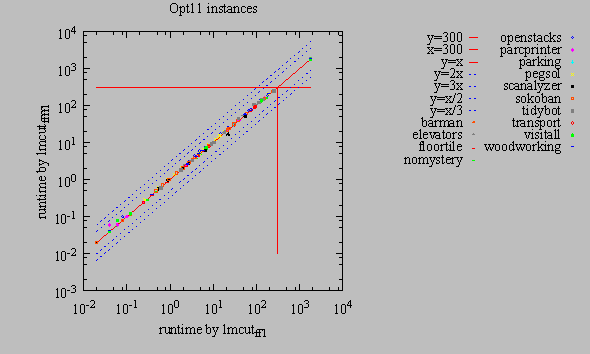
\includegraphics{tables/opt11-time-lmcut_ff-lmcut_ffff.pdf}
 \caption{Comparison of runtime on problems solved by both single FIFO search engine (ff) and a MultiSearch engine with 2 different instances of the same FIFO engine (ffff). The runtime difference was on average below a factor of x1.1, if we ignore the subsecond differences.}
 \label{ffff}
\end{figure}

Next, we evaluated our MultiSearch
strategy with selective combinations of two or three tiebreakings.
The configuration shown as ``lmcut m2'', ``lmcut m3'', ``mands m2'',
``lmcut m3'' are respectively the portfolio of
$[[\ld,\fifo], [\rd,\lifo]]$, $[[\ld,\fifo], [\ld,\ro], [\rd,\lifo]]$,
$[[\ld,\fifo],[\rd,\ro]]$, $[[\ld,\fifo],[\rd,\ro],[\ld,\lifo]]$. These
portfolios are hand-tuned.
% LOP is able to avoid the accidental bias
Results in \reftbl{portfolio-coverage}
shows a significant improvements compared to the results by each search
engine alone.
% 
Also, \refig{portfolio-runtime} shows the number of evaluations of these
tiebreakings compared to each search engine alone.  It shows that
MultiSearch acutally follows the expected behavior and the theoretical
bounds: the evaluation never exceeds twice/thirds of the single
search engine.

\begin{table}[htb]
 \centering \relsize{-2}
 \begin{tabular}{|c|c|c|c|c|c|}
\hline               
 Domain & \rotatebox[origin=l]{90}{${\mbox{lmcut}}_{\mbox{${\mbox{ld}}_{\mbox{fifo}}$}}$}   & \rotatebox[origin=l]{90}{${\mbox{lmcut}}_{\mbox{${\mbox{ld}}_{\mbox{random}}$}}$}   & \rotatebox[origin=l]{90}{${\mbox{lmcut}}_{\mbox{${\mbox{rd}}_{\mbox{lifo}}$}}$}   & \rotatebox[origin=l]{90}{${\mbox{lmcut}}_{\mbox{m2}}$}   & \rotatebox[origin=l]{90}{${\mbox{lmcut}}_{\mbox{m3}}$}    \\
\hline               
 sum(1104) &  \textbf{568} &  565 &  567 &  565 &  566  \\
\hline               
 {\relsize{-1}airport(50)} &  \textbf{27} &  25 &  26 &  26 &  26  \\
 {\relsize{-1}cybersec(19)} &  \textbf{3} &  \textbf{3} &  \textbf{3} &  2 &  \textbf{3}  \\
 {\relsize{-1}mystery(30)} &  \textbf{16} &  15 &  \textbf{16} &  15 &  15 \\
\hline
 sum(380) &  177 &  173 &  167 &  \textbf{180} &  177  \\
\hline               
 {\relsize{-1}airport-fuel(20)} &  14 &  13 &  \textbf{15} &  14 &  14  \\
 {\relsize{-1}driverlog-fuel(20)} &  7 &  7 &  \textbf{8} &  7 &  \textbf{8}  \\
 {\relsize{-1}logistics00-fuel(28)} &  \textbf{16} &  15 &  \textbf{16} &  15 &  15  \\
 {\relsize{-1}miconic-up(30)} &  20 &  20 &  18 &  \textbf{21} &  20  \\
 {\relsize{-1}mprime-succumb(35)} &  25 &  23 &  15 &  \textbf{28} &  25  \\
 {\relsize{-1}pathways-fuel(30)} &  4 &  4 &  \textbf{5} &  4 &  \textbf{5}  \\
 {\relsize{-1}tpp-fuel(30)} &  \textbf{11} &  \textbf{11} &  10 &  \textbf{11} &  10 \\
\hline
 sum(260) &  135 &  \textbf{137} &  127 &  134 &  133  \\
\hline               
 {\relsize{-1}blocks-stack(20)} &  \textbf{18} &  \textbf{18} &  17 &  \textbf{18} &  17  \\
 {\relsize{-1}elevators-up(20)} &  \textbf{11} &  \textbf{11} &  \textbf{11} &  9 &  10  \\
 {\relsize{-1}freecell-move(20)} &  \textbf{20} &  \textbf{20} &  18 &  \textbf{20} &  \textbf{20}  \\
 {\relsize{-1}gripper-move(20)} &  \textbf{7} &  6 &  \textbf{7} &  6 &  6  \\
 {\relsize{-1}mystery-feast(20)} &  6 &  6 &  \textbf{7} &  6 &  6  \\
 {\relsize{-1}pipesnt-pushstart(20)} &  \textbf{10} &  \textbf{10} &  8 &  \textbf{10} &  \textbf{10}  \\
 {\relsize{-1}pipesworld-pushend(20)} &  5 &  \textbf{6} &  3 &  5 &  5  \\
 {\relsize{-1}sokoban-pushgoal(20)} &  17 &  17 &  \textbf{18} &  17 &  17  \\
 {\relsize{-1}storage-lift(20)} &  \textbf{6} &  5 &  4 &  \textbf{6} &  \textbf{6}  \\
 {\relsize{-1}woodworking-cut(20)} &  7 &  \textbf{10} &  6 &  9 &  8 \\
\hline
 total(1744) &  \textbf{880} &  875 &  861 &  879 &  876 \\
\hline
\end{tabular}

 \caption{Coverage results comparing some LOP combinations and the
 single strategies under the portfolio. }
 \label{portfolio-coverage}
\end{table}

\begin{figure}[htb]
 \centering
 \relsize{-2}
 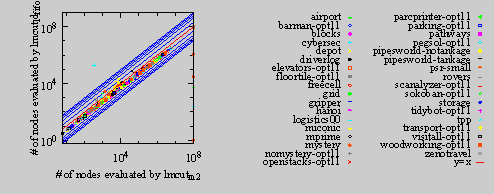
\includegraphics{tables/aaai16-5min/aaai16prelim3/evaluated-lmcut_m2-lmcut_ld_fifo.pdf}
 % 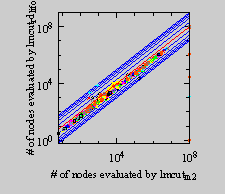
\includegraphics{tables/aaai16-5min/aaai16prelim3/evaluated-nokey-lmcut_m2-lmcut_rd_lifo.pdf}
 \caption{Runtime comparson between MultiSearch (X,Y,Z) and single strategies.}
 \label{portfolio-runtime}
\end{figure}


\section{Related Work}
\label{sec-4}

Previous work on escaping search space plateaus has focused on non-admissible search.
DBFS \cite{imai2011novel} is a technique which adds stochastic
backtracking to Greedy Best First Search to avoid being misdirected by the
heuristic function. Type based bucket \cite{xie14type} 
classifies the plateau of GBFS according to the $[g,h]$ pair.
Marvin \cite{Coles07} learns plateau-escaping macros from the Enhanced
Hill Climbing phase of the FF planner \cite{Hoffmann01} and later uses
these macros to escape the plateau.  However, to our knowledge, the
similar research on optimal planning was hardly located.

The PLUSONE cost-type is  non-admissible search technique in the LAMA planner \cite{richter2010lama}
which increases every action costs by 1.
Using PLUSONE, three successive
applications of zero-cost operators have cost 3, and two
applications have cost 2, and smaller cost is preferred, just as
\astar always expands the node with smaller $f$-value.
This explicitly targeted zero-cost actions observed in Openstacks,
and resulted in a significantly better performance in IPC-6.

The major difference of our depth-based tiebreaking from PLUSONE
strategy is twofold.  First, depth-based tiebreaking is admissible, because 
unlike PLUSONE, action costs are not modified.
Also, \emph{we do not always favor smaller depth over
larger depth}. LAMA treats the increased cost as the part of
sorting criteria. In contrast, it happens only in FirstDepth configuration in our case.

%% this will invoke a request from the reviewers to compare ours against it
%% * True, but people who know LAMA/FD are likely to demand some kind of comparison with alternating queues and preferred queues whether we mention  it or not.
%% Probably better to preemptively settle these questions rather than risking difficult questions during rebuttal.
TODO: other FD/LAMA comparisons: alternating queues vs LOP,   preferred queues vs depth-based tie-breaking.

% Another technique in LAMA is \emph{preferred operator queue},
% which is a technique that favors those actions which decreased the
% smallest $h$ value during the search.

TODO:  lazy A* vs LOP -- LazyA* combines multiple heuristics h1,h2 with low-overhead. However, if there is no dominance between h1,h2, behavior is different than h2; in contrast, LOP guarantees conservative behavior.

% It's not clear what these techniques have in common, except that they are all orthogonal to heuristics,
% If that's the case, then there's no need to cite them in this paper -- there's no reason why these particular techniques
% are more relevant to this paper than hundreds of other techniques that are orthogonal to heuristics.
%% In admissible planning,
%% \emph{Symmetry Breaking}
%% \cite{Fox1998,pochter2011exploiting,domshlak2013symmetry} is the search
%% technique that tries to prune the states with symmetric
%% paths. \emph{Partial Order Reduction}
%% % , \emph{Strong Stubbern Sets} and \emph{Expansion Core} are
%% is also a technique which prunes the
%% intermediate states that reach to the same goal using the different
%% orders of same actions. \emph{Dominance Pruning} \cite{hall2013faster} is a
%% technique which prunes a state if it can be proven to be worse than the other nodes.
%% % 
%% These are usually not considered an attempt to improve the heuristic
%% estimates, however, in terms of \emph{Path-dependent globally admissible
%% heurisitics} \cite{karpas2012optimal}, a class of heuristics which is
%% admissible only on a particular optimal path, generalizes the above
%% techniques as assigining an infinite cost to some nodes on the other optimal paths.
%% % 
%% % From a slightly different category, Pathmax \cite{mero1984heuristic} and
%% % Bidirectional Pathmax \cite{felner2011inconsistent} are the techniques
%% % which converts an inconsistent heuristics into non-decreasing,
%% % consistent heuristics.
%% Thus, in a broad term, all of these methods are the
%% attempts to improve the heuristic estimates.
%% % Although in some particular
%% % case they may be able to return a perfect heuristics, they are still not
%% % always a perfect heuristics, implying that the plateau is unavoidable.
%% In contrast, our tiebreaking techniques aims specifically at the case
%% where the plateau is encountered and the planners are forced to run a
%% knowledge-free search.

$LA^*$ \cite{stern2010look} is an extension of \astar which employs a
\emph{lookahead} to each expansion of a node. Lookahead is a depth first
search from the frontier node limited to a particular depth $k$. When
$k=0$, called $LA^*_0$ in their paper, the greedy expansion reaches only within
the same $f$-value. It is the same as LastDepth strategy in our
case, but there is no mention comparing $LA^*_0$ to tiebreaking strategy.

\citeauthor{Hoffmann05} gives a detailed analysis of the
structure of the search space in the benchmark domains in \citeyear{Hoffmann05}
\cite{Hoffmann05,Hoffmann14}. 
TODO: relationship to line of work by Hoffmann on search topology / plateau analysis? 



\section{Conclusion}

In this paper, we proposed two novel tie-braking methods for the admissible search using \astar. We empirically showed that they improve the performance on various domains, and they are heuristic-agnostic improvements. We showed that they have a significant impact on the final step of the search in large plateau.
 % when the distribution of optimal solutions is not uniform within the open list.
% We also showed that this nonuniform distribution still appears when we have almost-perfect % heuristics.

Our method differs from the pruning techniques because we actually
do not prune any states, nor from the other general improvements to the
heuristic accuracy because we just change the evaluation order within the
same $f$, yet it address the fundamental problems in the limitation of
heuristic forward search.  Future work includes a development of learning
technique for adaptively altering the search behavior in the plateau.



